\documentclass[border=10pt]{standalone}
\usepackage{tikz}
\usetikzlibrary{positioning, fit, arrows.meta, calc, decorations.pathreplacing}

\definecolor{coreblue}{HTML}{DBEAFE}
\definecolor{coreborder}{HTML}{3B82F6}
\definecolor{l1color}{HTML}{FEF3C7}
\definecolor{l1border}{HTML}{F59E0B}
\definecolor{l2color}{HTML}{D1FAE5}
\definecolor{l2border}{HTML}{10B981}
\definecolor{l3color}{HTML}{EDE9FE}
\definecolor{l3border}{HTML}{8B5CF6}
\definecolor{htlink}{HTML}{DC2626}
\definecolor{crosscore}{HTML}{2563EB}

\begin{document}
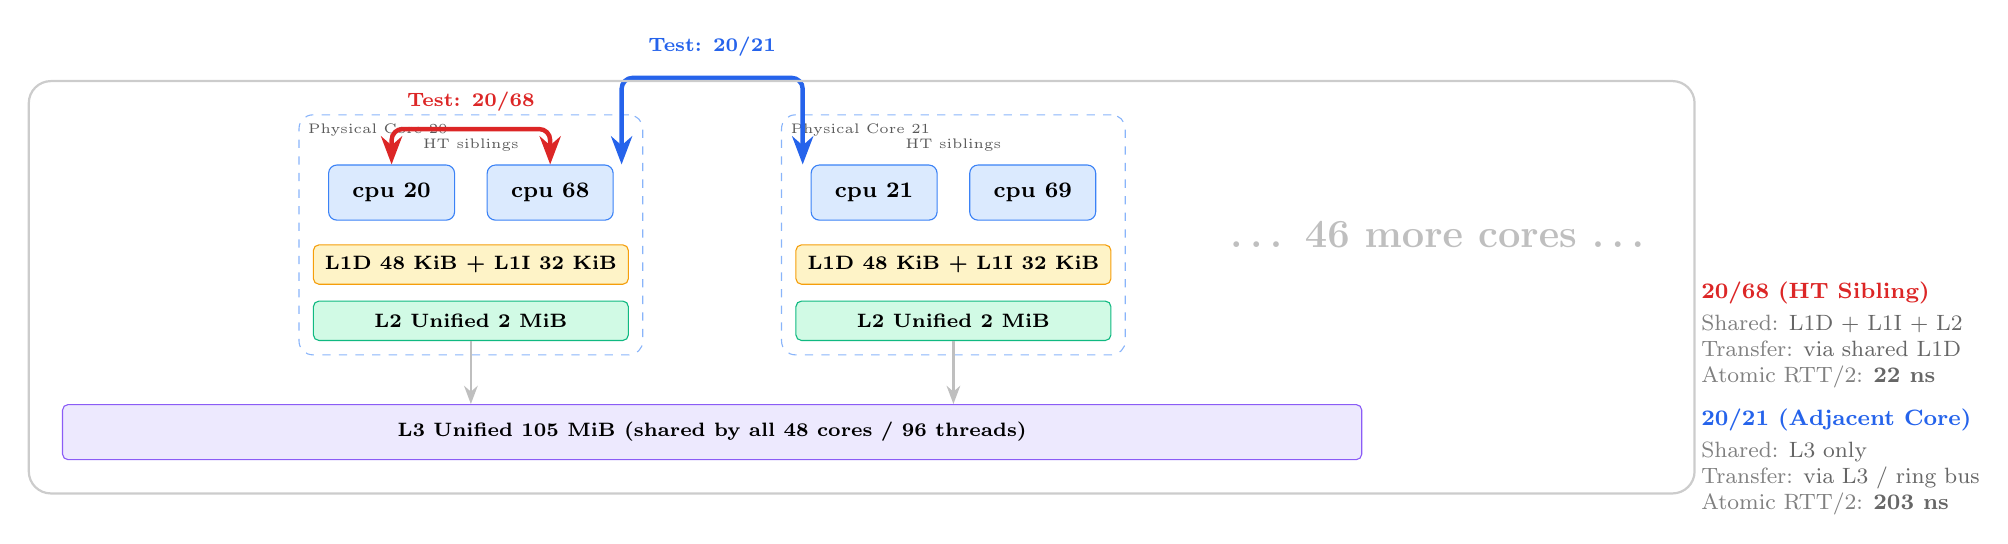
\begin{tikzpicture}[
    >=Stealth,
    core/.style={
        draw=coreborder, fill=coreblue, rounded corners=3pt,
        minimum width=1.6cm, minimum height=0.7cm,
        font=\footnotesize\bfseries
    },
    cache/.style={
        rounded corners=2pt, font=\scriptsize\bfseries, align=center,
        minimum height=0.5cm
    },
    l1/.style={cache, draw=l1border, fill=l1color},
    l2/.style={cache, draw=l2border, fill=l2color},
    l3/.style={cache, draw=l3border, fill=l3color},
    label/.style={font=\tiny, text=gray!70!black},
]

% =====================================================================
% Physical Core 20 (HT: cpu20 + cpu68)
% =====================================================================
\node[core] (cpu20) {cpu 20};
\node[core, right=0.4cm of cpu20] (cpu68) {cpu 68};

\node[label, above=0.05cm of $(cpu20.north)!0.5!(cpu68.north)$] (ht20label) {HT siblings};

% L1D + L1I shared
\node[l1, below=0.3cm of $(cpu20.south)!0.5!(cpu68.south)$, minimum width=4cm]
    (l1d20) {L1D 48 KiB + L1I 32 KiB};

% L2 shared
\node[l2, below=0.2cm of l1d20, minimum width=4cm]
    (l220) {L2 Unified 2 MiB};

% Physical core box
\node[draw=coreborder!60, dashed, rounded corners=5pt,
    fit=(cpu20)(cpu68)(ht20label)(l220), inner sep=5pt] (pcore20) {};
\node[label, anchor=north west] at (pcore20.north west) {Physical Core 20};

% =====================================================================
% Physical Core 21 (HT: cpu21 + cpu69)
% =====================================================================
\node[core, right=2.5cm of cpu68] (cpu21) {cpu 21};
\node[core, right=0.4cm of cpu21] (cpu69) {cpu 69};

\node[label, above=0.05cm of $(cpu21.north)!0.5!(cpu69.north)$] (ht21label) {HT siblings};

\node[l1, below=0.3cm of $(cpu21.south)!0.5!(cpu69.south)$, minimum width=4cm]
    (l1d21) {L1D 48 KiB + L1I 32 KiB};

\node[l2, below=0.2cm of l1d21, minimum width=4cm]
    (l221) {L2 Unified 2 MiB};

\node[draw=coreborder!60, dashed, rounded corners=5pt,
    fit=(cpu21)(cpu69)(ht21label)(l221), inner sep=5pt] (pcore21) {};
\node[label, anchor=north west] at (pcore21.north west) {Physical Core 21};

% =====================================================================
% Dots for remaining cores
% =====================================================================
\node[right=1.2cm of pcore21, font=\Large\bfseries, text=gray!50] (dots) {\ldots\ 46 more cores\ \ldots};

% =====================================================================
% L3 shared across all cores
% =====================================================================
\node[l3, below=0.8cm of $(l220.south)!0.5!(l221.south)$,
    minimum width=16.5cm, minimum height=0.7cm]
    (l3) {L3 Unified 105 MiB (shared by all 48 cores / 96 threads)};

% Connect L2 to L3
\draw[->, gray!50, thick] (l220.south) -- (l3.north -| l220);
\draw[->, gray!50, thick] (l221.south) -- (l3.north -| l221);

% =====================================================================
% Benchmark annotations
% =====================================================================

% HT sibling arrow (cpu20 <-> cpu68)
\draw[htlink, ultra thick, <->, rounded corners]
    (cpu20.north) -- ++(0, 0.45) -| (cpu68.north);
\node[font=\scriptsize\bfseries, text=htlink, above=0.55cm of $(cpu20.north)!0.5!(cpu68.north)$]
    {Test: 20/68};

% Cross-core arrow (cpu20 <-> cpu21)
\draw[crosscore, ultra thick, <->, rounded corners]
    (cpu68.north east) ++(0.1, 0) -- ++(0, 1.1) -| ([xshift=-0.1cm]cpu21.north west);
\node[font=\scriptsize\bfseries, text=crosscore, above=1.25cm of $(cpu68.north)!0.5!(cpu21.north)$]
    {Test: 20/21};

% =====================================================================
% Latency annotations (right side)
% =====================================================================
\node[anchor=north west, font=\footnotesize, text=gray!80!black,
    align=left, inner sep=0] at ([xshift=0.5cm, yshift=-0.3cm]dots.south east) {
    \textbf{\textcolor{htlink}{20/68 (HT Sibling)}} \\[2pt]
    \textcolor{gray}{Shared:} L1D + L1I + L2 \\
    \textcolor{gray}{Transfer:} via shared L1D \\
    \textcolor{gray}{Atomic RTT/2:} \textbf{22 ns} \\[6pt]
    \textbf{\textcolor{crosscore}{20/21 (Adjacent Core)}} \\[2pt]
    \textcolor{gray}{Shared:} L3 only \\
    \textcolor{gray}{Transfer:} via L3 / ring bus \\
    \textcolor{gray}{Atomic RTT/2:} \textbf{203 ns}
};

% =====================================================================
% Socket box
% =====================================================================
\node[draw=gray!40, thick, rounded corners=8pt,
    fit=(pcore20)(pcore21)(l3)(dots)(ht20label), inner sep=12pt,
    label={[font=\small\bfseries, text=gray!70!black]above:Intel Xeon Platinum 8488C --- 1 Socket, 1 CPU, 48 Cores, 96 Threads (no cross-socket / UPI)}] {};

\end{tikzpicture}
\end{document}
